\documentclass{article}
\usepackage{fullpage}
\usepackage{amsmath,amssymb,amsthm}
\usepackage[hidelinks]{hyperref}
\usepackage{graphicx}
\usepackage[utf8]{inputenc}
\usepackage{xcolor}
\usepackage{natbib}
% \usepackage{subcaption}
\usepackage{lineno}

\bibliographystyle{plainnat}

\newcommand{\comdist}{\widetilde{R}}
\newcommand{\comdistfn}{\widetilde{\mathcal{R}}}

\newcommand{\R}{\mathbb{R}}
\newcommand{\norm}[1]{\left\lVert#1\right\rVert}
\DeclareMathOperator{\var}{\mathop{\mbox{Var}}}
\DeclareMathOperator{\cov}{\mathop{\mbox{Cov}}}
\DeclareMathOperator{\diag}{\mathop{\mbox{diag}}}
\renewcommand{\P}{\mathbb{P}}
\newcommand{\E}{\mathbb{E}}
\newcommand{\given}{\,\vert\,}
\newcommand{\supp}{\mathop{\mbox{supp}}}
\newcommand{\sgn}{\mathop{\mbox{sgn}}}
\newcommand{\PP}[1]{\P\!\left\{#1\right\}}
\newcommand{\bone}{\mathbf{1}}

\newcommand{\plr}[1]{{\em \color{blue} #1}}

\begin{document}


\section*{Application to the Mojave Desert Tortoise}

The Mojave desert tortoise (\textit{Gopherus agassizii})
lives across much of the Mojave desert of California and Nevada,
separated from its sister taxa, \textit{Gopherus morofkaii} by the Colorado river.
We applied our method to genomic distances calculated from
whole genome sequencing data of 271 individuals sampled from across much of the range,
reported in \citet{shaffer2017desert}.
We discretized the landscape into 13 regions based on watershed polygons
from the Watershed Boundary Dataset \citep{WBD}
(using WBD8 slightly modified by portions of WBD10 to improve contiguity of regions).
The resulting discretization,
overlaid on a map including tortoise sampling locations,
is shown in Figure \ref{fig:tort_land}.
Since the regions vary substantially in size, 
and may vary substantially in population density, 
we do not assume that coalescence rates are the same everywhere, 
which gives 13 coalescence rates;
combined with the 50 migration parameters between each pair of adjacent regions
we have a total of 63 unknown parameters
(and 91 equations).

Posterior distributions of the parameters are shown in Figure \ref{fig:tort_post}.
There is substantial variation in the gene flow rates 
but not the coalescence rates, 
with the exception of region 4, which seems to have a relatively slow coalescence rate.
This is not too surprising given its large area and central location.
Gene flow rates are low across mountainous boundaries:
for instance, regions 1 and 4 are separated by the Paiute and Castle mountains,
and regions 4 and 12 are separated by the Providence and Granite mountains.
% and regions 1 and 9 are separated by the New York and McCollough mountains.
On the other hand, there is a large, mostly open bajada connecting areas 9 and 13, 
and we infer high rates of migration between the two regions.
The coalescence time model provides a good fit to the data,
much better than was obtained by commute times, either \plr{in this paper??}
or using the resistance distance method of \citet{shaffer2017desert}
(Figure \ref{fig:tort_h_comp}).

The most biologically interesting aspects
are the strong asymmetries, for instance between region 9 and regions 11, 12, and 13.
These indicate that resistance-based methods may be strongly misled.
However, we cannot conclude from this analysis \emph{what} is leading to the observed asymmetries.
One explanation would be source-sink dynamics:
for instance, the observed bias in lineage movement could be observed 
if the tortoise fecundity in the Ivanpah valley in region 9
is higher than in the colder, higher-elevation regions to the north.
Or, it could be the result of a historical range expansion out of the area,
perhaps out of a more restricted range as climates changed after the last glacial maximum.
The presence of source-sink dynamics would be of great interest for tortoise conservation efforts,
but it is not clear from this analysis which explanation is more likely.
Some aspects of the results may even be the produced by sample configuration:
for instance, perhaps the inferred gene flow between regions 2 and 3 is low
simply because individuals sampled in region 3 are geographically far from region 2.

\begin{figure}
\centering
 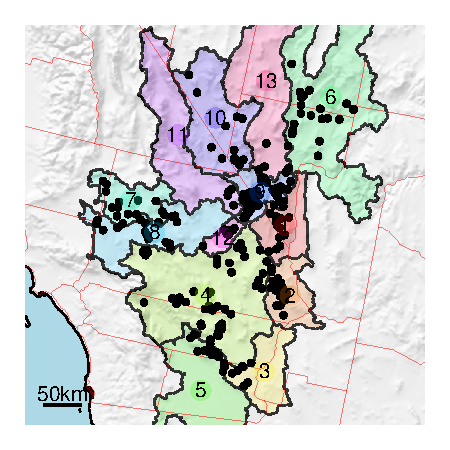
\includegraphics[width=0.45\textwidth]{figs/fancy_watershed_assignments}
 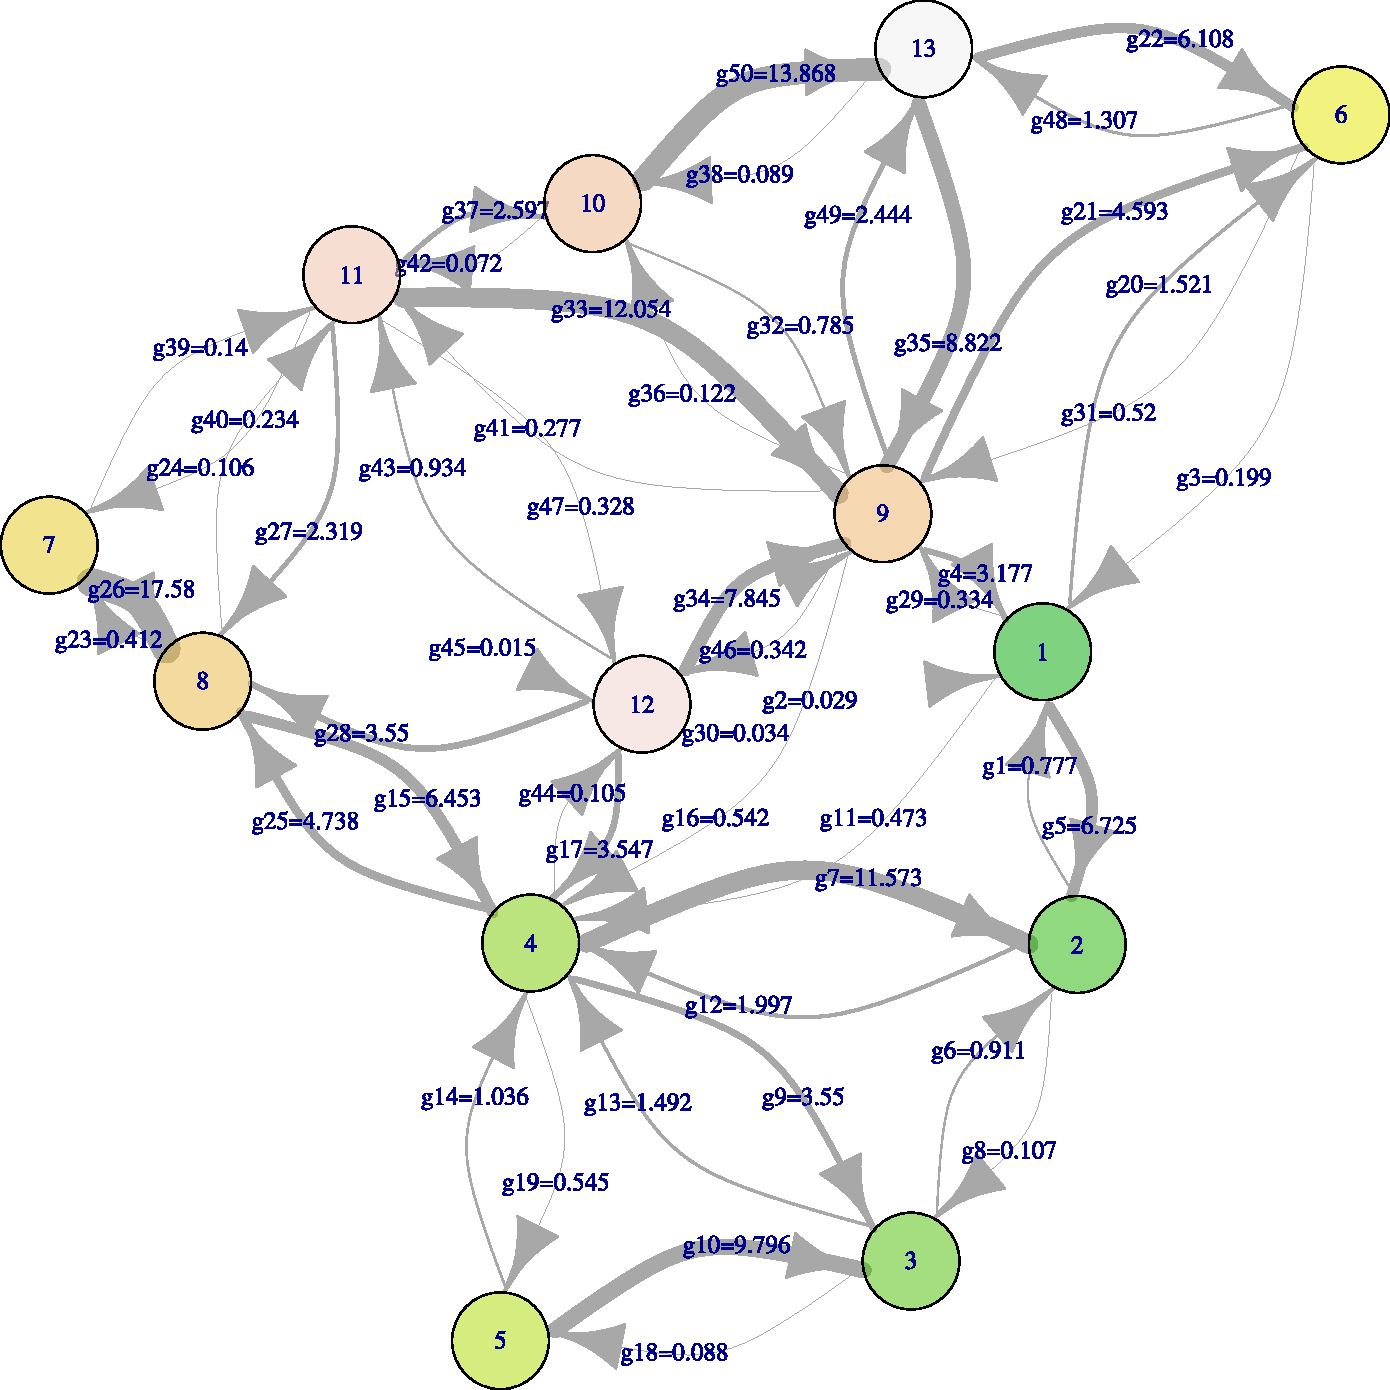
\includegraphics[width=0.45\textwidth]{figs/tort_graph_results}
\caption{Left: Locations of the sampled tortoises.
    \plr{remove bits on the other side of the Colorado}
    Right: Sample maximum posterior estimates 
    of movement rates.
    \plr{Note these are \emph{reverse-time} movement rates; we should reverse the arrows.}
    } \label{fig:tort_land}
\end{figure}

\begin{figure}
\centering
 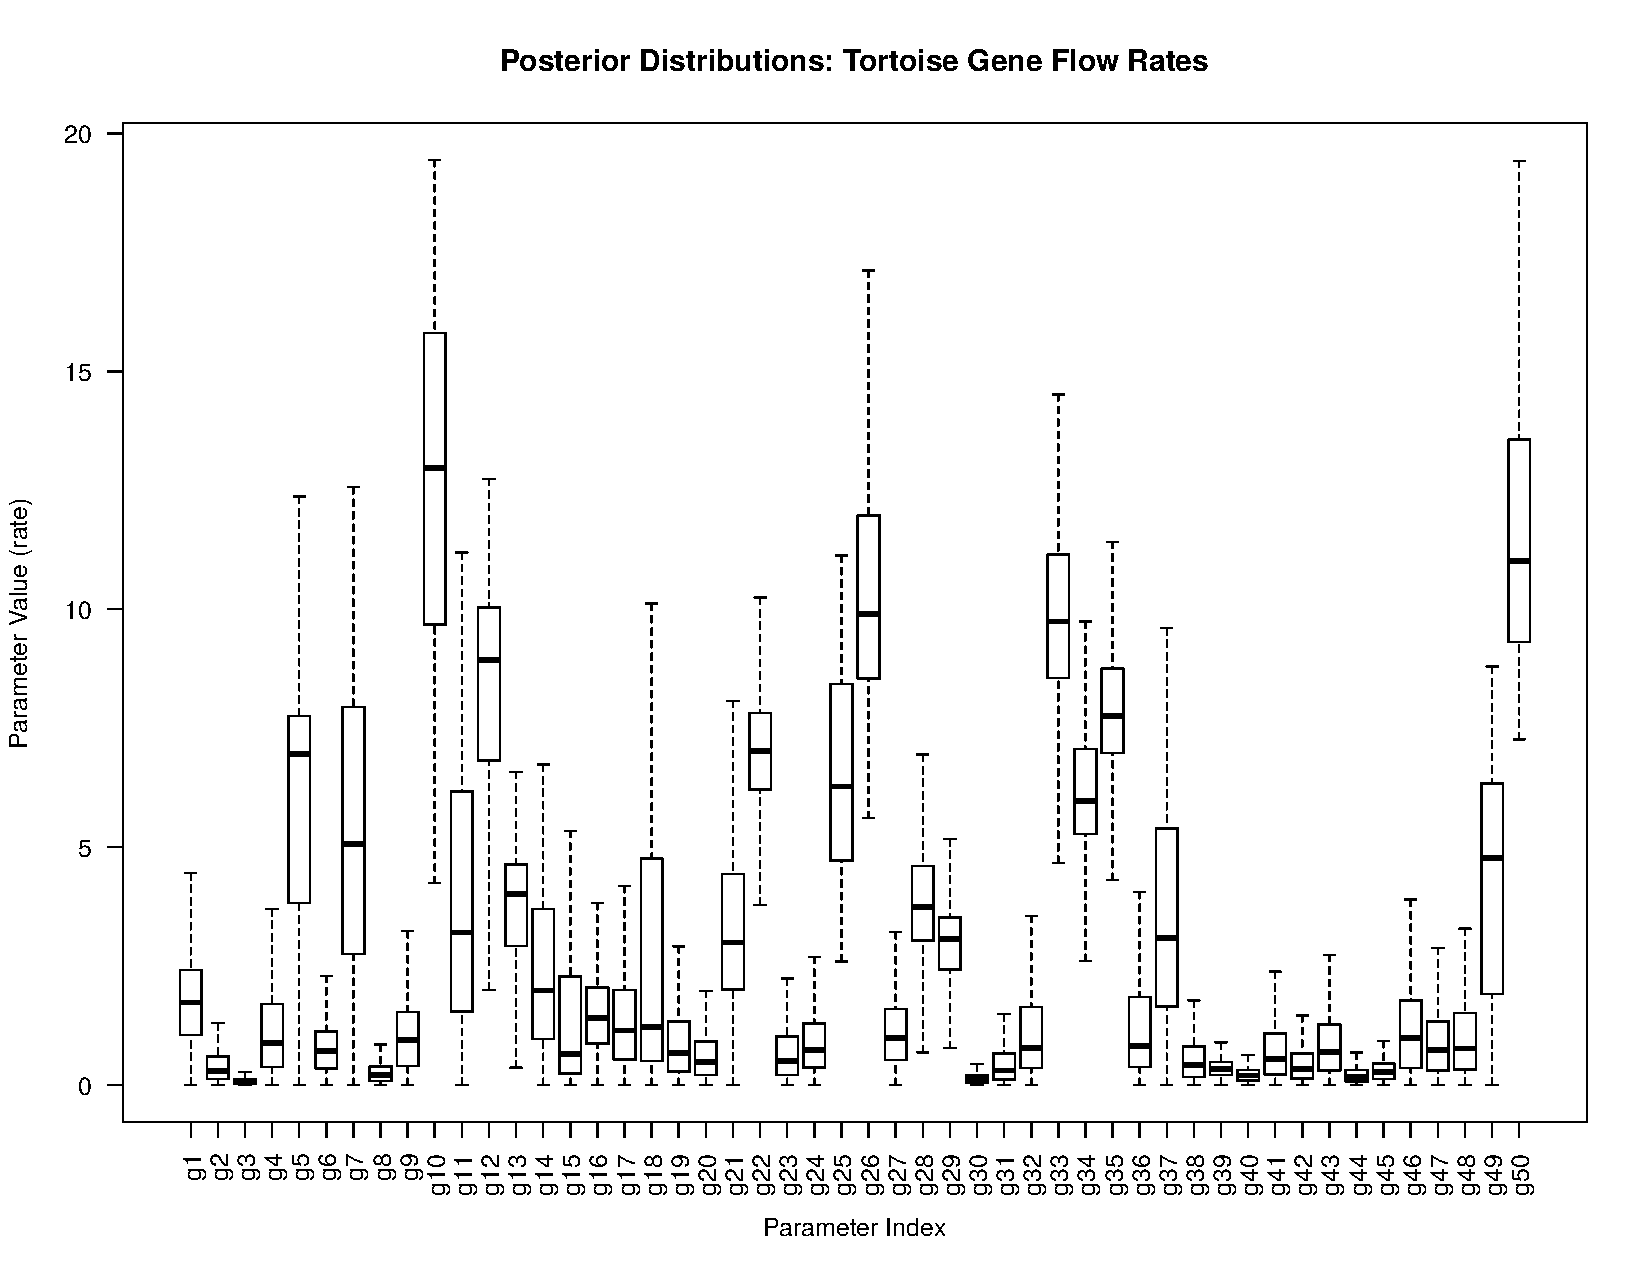
\includegraphics[width=0.8\textwidth]{figs/tort_post_g}
 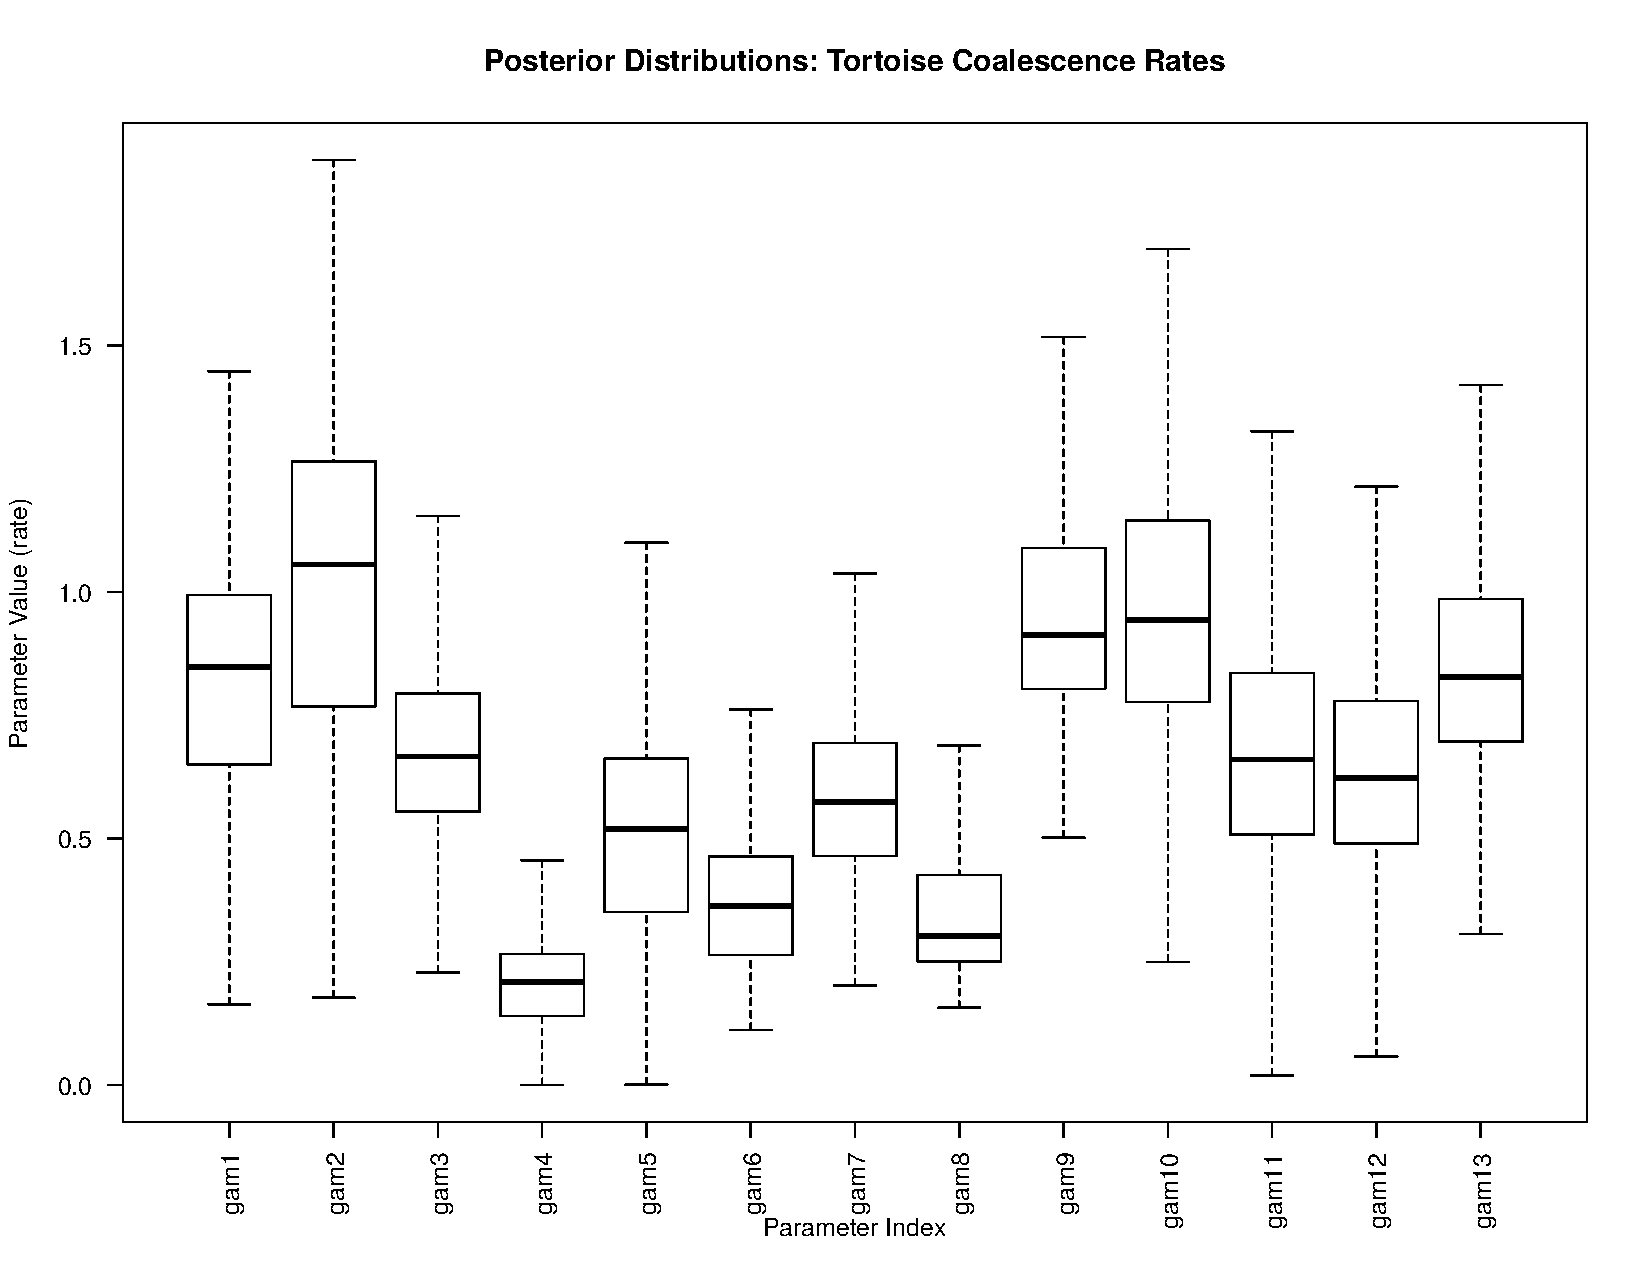
\includegraphics[width=0.8\textwidth]{figs/tort_post_gam}
\caption{
    Boxplots of the posterior distributions for 
    \textbf{(top)} movement rates, and
    \textbf{(bottom)} coalescence rates,
    for the Mojave desert tortoise data set.
    Parameters are labeled as in Figure \ref{fig:tort_land}.
    } \label{fig:tort_post}
\end{figure}

\begin{figure}
\centering
 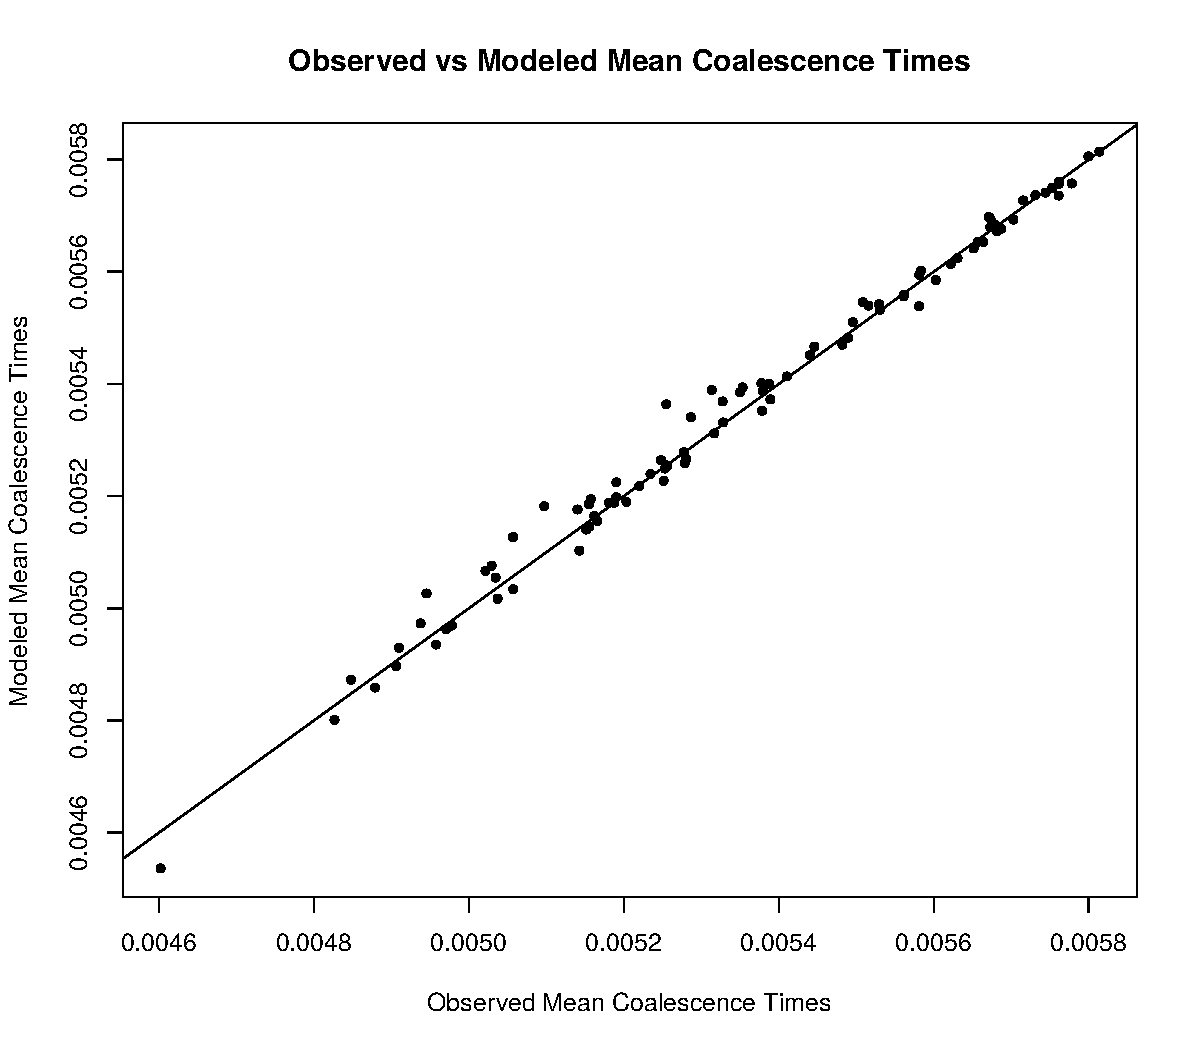
\includegraphics[scale=.8]{figs/tort_h_comp}
\caption{
    Mean coalescence times calculated from the sample maximum likelihood model parameters 
    plotted against the observed mean coalescence times calculated from the tortoise data, 
    measured in the mean of pairwise $\pi$.
    The mean absolute value relative differences between the two is 0.4\%.
    } \label{fig:tort_h_comp}
\end{figure}



\end{document}
